\chapter{React – A JavaScript library for building user interfaces}
\label{cha:react}

This chapter introduces the reader to the very popular and widespread front end library called ReactJS. It explains an essential part of React -- its rendering cycle -- which the reader needs to understand at least on a high level to be able to follow upcoming explanations of how the thesis project was implemented. Additionally, the paper elaborates the difference of how React uses declarative code to render data, whereas D3 uses an imperative API to render its data.

\section{Introduction to ReactJS}

The easiest way to find information about React is to visit its official website \footnote{https://reactjs.org}. There is a statement in \cite{React} up front that says: \begin{quote}\begin{english}React is a JavaScript library for building user interfaces.\end{english}\end{quote} which describes React very well. A Facebook engineer called Jordan Walke founded the library in 2011 as presented in \cite[05:30]{ReactFoundingVideo}. Walke wanted to create a tool that would improve the code quality of their internal tool called ''Facebook ads''. Up until then, Facebook continued to develop and use React internally, but since the year 2013, the project is entirely open source. Since the initial open-source release up until now, not only technical engineers of Facebook but also the React open source community itself have been maintaining the library. In late 2017 Facebook even changed React's BSD license to the MIT license, which is even better for the React community, as the MIT license has lesser restrictions than the BSD license.

According to \cite{React} Facebook sees React as a declarative and component-based library. However, a question might come to mind: ''What exactly does it mean for a library to be declarative and component-based?''. The answer to this question might be more straightforward than initially anticipated. In \cite{lloyd1994practical} declarative programming is described as a programming pattern, that expresses the logic of a program without describing its control flow. This means that the actual code only describes what has to be computed not necessarily how it should be done exactly by stating every action explicitly via a function call for example. Declarative programming can be understood as a layer of abstraction, that makes software easier to understand for readers of the code. Declarative programming is therefore very different from the imperative programming pattern described in chapter \ref{cha:d3js}. React's approach of handling the presentation layer is declarative since its API lets developers describe how the application has to look like at any given data variation, which is quite the contrary to D3's API as it can be read in \ref{cha:d3js}. Further information about React's API can be found in section \ref{sec:reactApi} though.

Enabling developers to create a highly component oriented architecture in their software is a fundamental aspect of React as well. Using a component-based library can increase productivity a tremendous amount. However, what does it mean for a library to favor component based architecture? After the initial setup of some boilerplate code, React makes it exceptionally easy to reuse existing components in the codebase to allow even faster development cycles. Once standard input components like buttons or text fields and layout components like page or header components are implemented, they can be reused throughout the whole app; thus significant progress can be achieved in a very short amount of time. Components can be manipulated by passing different properties, which might result in different presentation results of the components. More in-depth information about how React handles components and its props can be found in section \ref{sec:reactApi}.

React components can have multiple applications. There are presentational components for example which are pure functions that simply represent the current application state. Though there are also stateful Components which can hold some application state and react to state changes accordingly via rendering again. React however makes no assumptions about the technology stack that is used in a project as \cite{React} claims. This means that users of the library can decide for themselves if they want to use the built-in state management functionality or if they want to use a third-party library for solving specific problems like global application state for example.

The documentation in \cite[/docs]{React} claims that the library makes use of a so-called ''virtual DOM''. This means that React keeps track of its state data to prevent unnecessary writes to the actual DOM object. JavaScript performs exceptionally well when handling pure JavaScript objects in memory. Keeping the DOM tree of the application in the JavaScript engine's heap as a representation of objects enables React to apply data updates this so-called virtual DOM, then diff the newly applied data with the old tree to then being able to decide what DOM nodes need to be rewritten. Writing or committing to the DOM is the most expensive type of work in the browser, so React tries to keep DOM manipulating actions to a minimum. The React team calls the diffing algorithm ''reconciliation algorithm''. It would go out of the scope of this paper to go more in depth of the algorithm, so it is recommended to read about React's reconciliation algorithm in its documentation \cite[/docs]{React}.

React is a view layer that favors unidirectional data-flow. Every time the application state changes, the whole new data object is passed to React again. As mentioned in \cite[6:50]{ReactFoundingVideo}, the speaker describes the functionality very well via explaining React as a simplified function that could look like this: \texttt{f(data) = UI}. Hence, React can be seen as the view layer that handles presentation as a function of state and data. Once the data has updated the virtual dom, the virtual dom is then passed to React's reconciliation algorithm which then determines if any nodes have to be changed on the real DOM. If there would be a React component that always renders the same \texttt{<div>} with the same data, rendering that very component multiple times would not result in React writing multiple DOM nodes to the browser. The reconciliation algorithm sees that the virtual dom matches the real dom in this case, which results in React not updating the real DOM. Of course, if the component's content is dynamic, the component sometimes has to be re-rendered according to the data changes. If some parts of the data stay the same even after being reapplied to a component, only newly added or removed nodes are committed to the DOM. Even though the reconciliation algorithm prevents expensive DOM operations, the algorithm itself can also be expensive. The documentation in \cite[/docs/optimizing-performance.html\#avoid-reconciliation]{React} advises developers to try to avoid reconciliation to improve performance.

Unidirectional data-flow implicitly means to React, that there is no data binding and no template language. The library only uses \texttt{React.createElement([element])} calls internally, which are hidden behind the so-called ''JSX'' JavaScript language extension. JSX will be explained more i depth in section \ref{sec:reactApi}. As mentioned before, React is just a pure idempotent function of its application state, which means that the same data always produces the same presentation. This also means if the application data has to be changed, a new ''patched'' version of the application data has to be created which then flows into the React render cycle again Unidirectional data-flow is also the reason why React works well with immutable data structures. This paper assumes that the reader knows about immutable data structures, but \cite{ImmutableJS} explains exceptionally well, what are Immutable data structures and how they're used in JavaScript. Going more in-depth on how React works well with immutable state would go out of the scope of this thesis though. It is just essential to know that every time the data change this triggers a whole new render cycle of React. The immutable data structures help React to work out changes in the data structure, as nested data object tree differences can be checked via a cheap equality check when using immutable data structures.

\section{Explaining the React API}
\label{sec:reactApi}

To follow performance discussions and elaborations about the thesis project's prototypes, a generally high-level understanding of the API is required. This section introduces the reader to React's public API. The section does not aim to be a tutorial on how to program React applications, but rather a high-level explanation of how the API works. Reading this section makes it easy to understand the differences and similarities of React and D3 and how the two libraries play together and how they're also completely different.

\subsection{JSX in general}

\begin{program}
\caption{Creating a React element with JSX} 
\label{prog:reactJsxElement}
\begin{JsCode}
const ReactElement = (
  <div className="hello-world">
    Hello <span className="important">World</span>!
  </div>
)
\end{JsCode}
\end{program}

\begin{program}
\caption{Creating a React element without JSX} 
\label{prog:reactJsxTranspiled}
\begin{JsCode}
var ReactElement = React.createElement(
  "div", 
  { className: "hello-world" }, 
  "Hello ", 
  React.createElement(
    "span", 
    { className: "important" }, 
    "World"
  ), 
  "!"
);
\end{JsCode}
\end{program}

Probably one of the most important aspects of React's API is the JavaScript language extension called ''JSX'' which simplifies the use of React greatly and produces much more readable code. The example in \ref{prog:reactJsxElement} shows an example React component that is written in JSX. Notice, that the class property has to be \texttt{className} instead of \texttt{class} as JSX is \emph{not} HTML, but extended JavaScript.

When looking at the transpiled output in \ref{prog:reactJsxTranspiled} it is clear how JSX helps to reduce the amount of code and how it greatly improves readablity. The code in \ref{prog:reactJsxTranspiled} also shows that React is just a big composition of \texttt{React.createElement([element])} calls under the hood. When writing JSX code, in reality it is writing declarative code that is just a functional composition of React components. Notice, how the createElement function takes up to 3 parameters as documented in \cite[/docs/react-api.html]{React}. The first parameter being the element type (the type can also be a custom user or third party component), the second parameter being the element's properties and the third parameter being the compoennt's children. The third parameter is the one which makes it possible to compose many React components together.

Because JSX is a language extension, a transpile step is needed in order to produce production code. The common tool to use is called ''Babel''. There is a caption in \cite{Babel} that says: \begin{quote}\begin{english}Use next generation JavaScript today.\end{english}\end{quote} The documentation in \cite[/docs/en]{Babel} explains, how modern JavaScript features can be used in any JavaScript project. The code which includes those modern features is normalized and transpiled by Babel to also work in older browsers. The tool accomplishes this by transforming the JavaScript code via its core implementation but also via some third party plugins. A babel plugin has been created to transform JSX components into the syntax that can be seen in the code in \ref{prog:reactJsxTranspiled}. Just as a sidenote, altough JSX became popular in conjunction with React, there are also other web technologies that make use of JSX like Vue.js \footnote{https://vuejs.org/} for example.

\subsection{Explaining React components}
\label{sec:reactComponents}

\begin{program}
\caption{Simple example of a React component and its usage} 
\label{prog:reactHelloWorld}
\begin{JsCode}
const HelloComponent = props => {
  const name = props.name;
  return <div>Hello World to {name ? name : "you"}!</div>;
};

const PageComponent = props => {
  props.customFn("I get passed to the handler function!");
  return (
    <div>
      <h1>{props.title}</h1>
      <div>{props.content}</div>
      here are my children: [{props.children}]
    </div>
  );
};

const App = () => {
  return (
    <PageComponent
      customFn={console.log}
      title="I render the title prop"
      content="I render the content prop"
    >
      <HelloComponent />
      <HelloComponent name={"Max"} />
    </PageComponent>
  );
};
\end{JsCode}
\end{program}

As mentioned before, React is a highly component oriented web technology. The example code in \ref{prog:reactHelloWorld} includes a sample presentational component called ''HelloComponent'' on line 1, a page layout component on line 6 and the base App component on line 17. The app renders the page layout coponent, passes a few props and then renders the HelloComponent twice inside the layout component. One time the HelloComponent receives the prop \texttt{name} and one time the property is omitted. The output of the hello world example can be seen in figure \ref{fig:reactHelloWorld}. The example in \ref{prog:reactHelloWorld} visualizes, how components can be reused throughout the application with different configurations and in different arrangements. The page layout component could be declared in its own file to be reused in every page of the app. Via props React provides a solid mechanism to control static state of the components that receive the props. 

It is of utmost importance to understand, that props -- once they're passed to a component -- are static and immutable inside the receiving component. Components that render props can be seen as pure functions that only render the props that they receive each render cycle. The props could thus be understood as the parameters of the pure functions.

\begin{figure}
  \centering
  
\includegraphics[width=0.35\columnwidth]{react001}
  \caption{React hello world sample output}
  \label{fig:reactHelloWorld}
\end{figure}

\begin{program}
\caption{Simple example of a React component and its usage} 
\label{prog:reactStatefulComponent}
\begin{JsCode}
const Count = props => (
  <div>
    <div>I render the count</div>
    <div>The count is currently {props.count}</div>
  </div>
);

class StatefulComponent extends React.Component {
  state = {
    count: 1
  };

  counterHandler = () => {
    this.setState(state => ({ count: state.count + 1 }));
  };

  render() {
    return (
      <div>
        <Count count={this.state.count} />
        <button onClick={this.counterHandler}>+1</button>
      </div>
    );
  }
}

const App = () => <StatefulComponent />;
\end{JsCode}
\end{program}

\begin{figure}
  \centering
  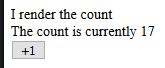
\includegraphics[width=0.25\columnwidth]{react002}
  \caption{React counter component output}
  \label{fig:reactCounterComponent}
\end{figure}

% what is state for the one component is immutable static prop for the other

%Another important aspect of React which is important for this project are its life cycle methods. Each component has a life cycle that will be executed on each rendering cycle. Developers can hook into those life cycle methods to implement some logic that should be executed after a component mounts or after a component was updated for example. The most well known life cycle methods of React are \texttt{componentDidMount()} or \texttt{componentDidUpdate()}.

\section{The difference between imperative and declarative APIs}


